\section{Engine}
\label{secengine}

\makeatletter
\newenvironment{myalign*}{%
\setlength{\mathindent}{0pt}%
\setlength{\abovedisplayskip}{-\baselineskip}%
\setlength{\abovedisplayshortskip}{\abovedisplayskip}%
\start@align\@ne\st@rredtrue\m@ne
}%
{\endalign}
\makeatother

\subsection{Mathematics}

Mathematics is an important part of any 3D rendering application. 
As there is little point in reinventing the wheel and many good mathematics libraries exist already, our implementation uses classes from 
jMonkeyEngine\footnote{\url{http://jmonkeyengine.com/}} for general tasks such a matrix multiplication. These libraries are mixed with additional classes and functions of our own for tasks that are more specific to our application
 or simply missing from jMonkeyEngine's implementation. For example the jMonkeyEngine matrix implementations have no methods for getting the basis vectors of a matrix or creating left handed look at matrices.

\subsubsection{Number spaces and matrices}
\label{numandmat}

We use 4x4 matrices to represent transformations in our engine. Such a matrix allows for rotating, scaling and translating world objects. It also allows for the creation of view and projection matrices as explained later. 
The diagrams from this section were adapted from \cite{matrixdiagref}.

\begin{figure}[!htbp]
  \begin{center}
    \leavevmode
    \ifpdf
      \includegraphics[width=0.7\textwidth]{matrices1}
    \fi
    \caption{4x4 matrix layout}
    \label{FigMatrices1}
  \end{center}
\end{figure}

\pagebreak
The 4x4 identity matrix looks as follows and geometrically it represents applying no transformation to an object.

\begin{figure}[!htbp]
  \begin{center}
    \leavevmode
    \ifpdf
      \includegraphics[width=0.7\textwidth]{matrices2}
    \fi
    \caption{4x4 identity matrix}
    \label{FigMatrices2}
  \end{center}
\end{figure}

Each object in the scene has a world matrix which represents how it is transformed from object space into world space. 
That is, an object's geometry is stored with respect to the origin and is transformed into its desired location in world space via this transformation. 
If a scene is completely static, the object could be pre-multiplied by this matrix to avoid having to perform a transformation on each render call. World space is in $([FP_{MIN},FP_{MAX}],[FP_{MIN},FP_{MAX}])$,
where $FP_{MIN}$ and $FP_{MIN}$ are the maximum and minimum numbers that can be stored by a floating point number of some known precision, in the case of our application double precision is used due to the scales involved.

\begin{figure}[!htbp]
  \begin{center}
    \leavevmode
    \ifpdf
      \includegraphics[width=0.7\textwidth]{matrices3}
    \fi
    \caption{4x4 world matrix}
    \label{FigMatrices3}
  \end{center}
\end{figure}

\pagebreak
The view matrix transforms world space into view space. 
The basis vectors of 3x3 submatrix of the view matrix define the viewing angle of the camera. 
These vectors transform the world basis vectors into the camera basis vectors. It will also translate coordinates depending on camera position. 
View space is in $([FP_{MIN},FP_{MAX}],[FP_{MIN},FP_{MAX}])$.

\begin{figure}[!htbp]
  \begin{center}
    \leavevmode
    \ifpdf
      \includegraphics[width=0.7\textwidth]{matrices4}
    \fi
    \caption{4x4 view matrix}
    \label{FigMatrices4}
  \end{center}
\end{figure}

The projection matrix transforms view space into screen space. As well as this, it defines a near and far clipping plane (any pixel that falls outside of those planes will not reach the pixel shader stage during render calls) and also adds perspective to view space. 
The perspective is based on a pre-defined field of view and the aspect ratio of the output window. Screen space is in $([-1,-1],[1,1])$.

\begin{figure}[!htbp]
  \begin{center}
    \leavevmode
    \ifpdf
      \includegraphics[width=0.7\textwidth]{matrices5}
    \fi
    \caption{4x4 projection matrix}
    \label{FigMatrices5}
  \end{center}
\end{figure}

\pagebreak
All of these matrices can be combined so that an object can be transformed from object space into screen space in a single step. This is what is most commonly done on the GPU shaders,
 although certain calculations will additionally require other information about a vertex besides its screen coordinates. An example would be lighting calculations which are performed in world space at the pixel shader stage.

\paragraph{Double space and float space}

The vast scale of the solar system requires that calculations are done using double precision, calculations done at such precision will be referred to as occuring in double space (that is, $Double space = [double]^3$).
A double precision floating point number allows the storing of 15 significant decimal places which is enough to store object information down to a scale of 1mm (Since Pluto is around $4.436*10^15$mm from the Sun
 and it is the most distance object that will be rendered). These values must be converted to single precision floating point numbers before sending them to the GPU, which will be referred to as converting to float space. 
 This conversion introduces precision problems when rendering the scene, the solutions used to combat this are discussed in \cref{precisionimpl}.

\subsubsection{Quaternions}

Quaternions are also used in the calculation of rotations on the CPU. 
This is due to the lower memory and performance cost associated with them when compared to 3x3 rotation matrices due to only having four floating point components rather than nine. 
The details of how and why quaternions work is beyond the scope of this report, but in essence they avoid the gimbal lock problem encountered if using Euler angles by defining a rotation around an axis vector by some scalar amount as opposed to a rotation about three angles (i.e. a rotation for each unit vector).

\pagebreak
\subsubsection{Camera}

The camera determines the user's view of the scene. This involves three main factors: the camera's position, rotation and perspective (represented by a view and project matrices - see \cref{numandmat}).
Our implementation splits these tasks between two classes. The base class deals only with the camera perspective, that is, generating the projection matrix. The class defines a value for the aspect ratio and field of view of the camera which determine the x and y scale values of the viewing frustum respectively. It additionally defines near and far clipping planes which limit the minimum and maximum distance of an object before it is not rendered. These four values combined can be used to find a projection matrix and the planes which comprise the view frustum.

\begin{figure}[!htbp]
  \begin{center}
    \leavevmode
    \ifpdf
      \includegraphics[width=0.75\textwidth]{perspect_diag}
    \fi
    \caption[Camera frustum]{Camera frustum\protect\footnotemark}
    \label{FigFrustumDiag}
  \end{center}
\end{figure}

\footnotetext{Source: \cite{viewfrusdiagref}}

The derived class adds the functionality for generating the view matrix which it does by combining a translation and rotation value. It also provides functions that allow for these values to be intuitively changed by the user. For example the move function takes a 3d value by which to move the camera and transforms the values from being relative to the Cartesian unit vectors to be relative to the basis vectors of the camera's rotation matrix. It also provides functions which handle user input, look at a particular object in the scene, save and restore a particular view and rotate the camera in place.

\pagebreak

\subsection{Scene graph}
\onehalfspacing
A scene graph is a data structure that is used to store information about the graphical scene in a hierarchical manner. 
The main classes involved in our scene graph are: Scene, Node3D and Entity3D. An entity represents an object in the world (which may or may not be renderable) and a node is an entity which can also have child entities. A scene stores a node which is the root of the entire scene to be rendered. Every entity has its own scale, translation and rotation. During a scene update, these values are used to assemble the local transformation matrix for the entity. The update procedure works recursively, and at each level the objects world matrix is also calculated based on the transformations of the parent entities and the object's local matrix.
Many scene graph implementations propagate the entire transformation matrices down the hierarchy, this implementation was not desirable for us as it would be awkward for example to define the rotation and scale of the Earth in terms of the Sun.
Instead the only value inherited from parents is the translation. This fits well with how data is provided in terms of the orbital and rotational properties of the solar bodies.

% Define block styles
\tikzstyle{decision} = [diamond, draw, fill=blue!20, 
    text width=4.5em, text badly centered, node distance=3cm, inner sep=0pt]
\tikzstyle{block} = [rectangle, draw, fill=blue!20, 
    text width=5em, text centered, rounded corners, minimum height=4em]
\tikzstyle{line} = [draw, -latex']
\tikzstyle{cloud} = [draw, align=center, ellipse,fill=red!20, node distance=3cm,
    minimum height=2em]
	
\singlespacing 
\begin{figure}[!htbp]
  \begin{center}
\begin{tikzpicture}[node distance = 3cm, auto]
    % Place nodes
    \node [block] (root) {Root node};
	\node [block, right=4cm of root] (nodediag) {Node};
	\node [cloud, below=0.75cm of nodediag] (entitydiag) {Entity};
	\node [block] (root) {Root node};
    \node [block, below=0.75cm of root] (sun) {Sol};
	\node [block, below=0.75cm of sun] (venus) {Venus};
	\node [cloud, left of=venus] (venuspath) {Path \\ (Venus)};
	\node [block, right of=venus] (earth) {Earth};
	\node [cloud, below=0.75cm of earth] (luna) {Luna};
	\node [cloud, right of=luna] (lunapath) {Path \\ (Luna)};
    % Draw edges
    \path [line] (root) -- (sun);
	\path [line] (sun) -- (venuspath);
	\path [line] (sun) -- (venus);
	\path [line] (sun) -- (earth);
	\path [line] (earth) -- (luna);
	\path [line] (earth) -- (lunapath);
\end{tikzpicture}
    \caption{Example of partial scene graph for the app}
    \label{FigSceneGraph}
  \end{center}
\end{figure}
\onehalfspacing
\pagebreak

\subsection{Geometry}

There are four main types of geometry used in the simulation, spheres, models, lines and planes. Spheres are used for the planets, their moons and Sol. These can be deformed with heightmaps \cref{heightmaps} if the camera is close enough for the difference to be discernible. Imported 3D models are used for the space ship the user can fly, they could also be used for asteroids but currently are not as not many accurate models are available. Lines are used to draw paths for the orbits of planets and moons as well as for tracing the path of the ship. Planes are used in a number of ways which are described in later sections including: \cref{bitmapfont}, \cref{starfield} and \cref{planetaryrings}. All geometries other than 3D models are algorithmically generated on program start-up.

\subsection{Intersection tests}

There is a need for intersection tests for both collision detection and render list queries (\cref{culling}). Collision detection prevents the user from being able to fly through planets and other galactic bodies. Our test is simple and gives bodies and the camera a containing boundary sphere, if the spheres intersect the camera is stopped from going any closer to the object. This option was chosen simply because sphere/sphere intersection tests are computationally simple. Render list queries test whether an object is in view before a GPU draw call is performed. Without such tests many times more geometry would be rendered than what is actually required so this technique is used on practically on all modern graphics applications of any real scope. The task is often performed on both the CPU and GPU, but due to the limitations on current mobile GPUs we do all such tests on the CPU.

\subsubsection{Frustum Culling}
\label{culling}

To cull objects, that is, to prevent them from being added to the render lists, we use a frustum test. Using the camera's view and projection matrices it is possible to calculate a frustum which represents the visible area. This frustum is stored as six planes which can then be used in calculations along with different bounding volumes to test for: containment, intersection or disjointness. In this case it does not matter whether or not an object intersects or is contained completely so the cases are treated as the same and result in an entity being added to the render list. The bounding volume we use for this test is a sphere since the calculations are the most simplistic and it is desirable to keep the load on the relatively unpowerful mobile CPUs at a minimum. 

\begin{figure}[!htbp]
  \begin{center}
    \leavevmode
    \ifpdf
      \includegraphics[width=0.65\textwidth]{frustum1}
    \fi
    \caption{Camera frustum}
    \label{FigFrustum}
  \end{center}
\end{figure}

\subsection{The render loop}

All renderable objects inherit the same interfaces which give rise the the following render loop:

\begin{enumerate}
\item Update - update the local and world matrices of objects with new rotations and scales (for example planets will call their orbit functions to get their new position). The camera will be tested for collisions as well.
\item Query - objects will be tested for visibility by comparing their bounding volumes with the camera frustum (\cref{culling}). If visible, they will be added to the render and post render lists.
\item Render - Objects added to the render list are then rendered. This is where the majority of the rendering work is done.
\item Post render - Objects in the post render list are sorted by distance to camera. This is to be used only for objects with transparency where the draw order is important. Examples include planet atmospheres (\cref{atmospheres}), planetary rings (\cref{planetaryrings}) and the corona of the Sun.   
\end{enumerate}

\subsection{Texture IO}

Due to the large number textures required to render the planets and their various moons to a high level detail some consideration needs to be given to how to load them. There are three main elements to this: loading the data, processing the data and uploading the data to the GPU. To minimise the number of disk reads required, some form of compression should be used. Ideally this compression format would be natively supported on the GPU to avoid having to perform decompression first before uploading. There is considerable variation in the texture compression formats supported by mobile GPUs, the normal workaround for this is simply to store textures in many formats and load the appropriate one for the platform required. However, due to the large number of textures required (for a mobile app), it would have used around 200MB of disk space to store all the textures in three different formats. Instead we opted just to store textures as JPEG for RGB and PNG for RGBA. The problem with these formats is that they do not store mipmaps (smaller resolution versions of the images used as the distance to an object increases). These are required in order to correctly render distant objects so the only option is to calculate them. Since JPEG and PNG have no native support on GPUs they must be uploaded in their decompressed form which will use more GPU memory. Finally, uploading data to the GPU is still fast even though data is being sent uncompressed. The resulting load time on a Samsung N7000 was around three seconds, we estimate this could be at least halved if a format with precomputed mipmaps and natively supported compression formats was used based on our experiments on the PC version described below.

\subsubsection{Direct draw surfaces}

On the PC version a loader was implemented that parses Direct Draw Surfaces (DDS) with textures compressed in the DXT1-DXT5 formats. These formats can support both RGB and RGBA formats and have native support on almost all modern desktop GPUs. They also have pre-generated mipmaps so there is no additional work to perform after loading. This resulted in the loading of textures on the PC version being many times faster than what was achieved for the Android version. The code is compatible with the Android version and if future mobile GPUs have native support for the format the app could benefit from significantly improved load times.

\subsection{GPU buffer management}

Since a large amount of geometry is involved in rendering the scene, particularly if a high star and asteroid count is being used, managing the index and vertex buffers as efficiently as possible is one of the keys to obtaining good performance. 

Firstly on the CPU side, one particular problem we found in earlier iterations of the application was that Android has very bad performance when it came to allocating instances of the java Buffer class. 
This operation was performed extensively for dynamic geometries such as bitmap font based text (\cref{bitmapfont}) and at the time as benchmarks on the PC version had shown that the performance cost was negligible when compared to draw calls, orbit calculations and scene updates. On Android however, updating the debug text was using about 25\% of the CPU time. 
This problem was solved by pre-allocating a Buffer instance and updating it if the new geometry to be stored was of equal or smaller size than what was previously stored. 
Only if the new geometry is larger should a new buffer allocated and this generally only occurs a few times soon after the application starts up.

\subsubsection{Vertex Buffer Objects and Index Buffer Objects}
\label{vboibo}

OGLES 2.0 also provides the ability to store buffers in GPU memory rather than in main memory via Vertex Buffer Objects (VBOs) and Index Buffer Objects (IBOs). These allow the upload of this data to be asynchronous via various specifications on buffer creation and also provide hints which allow for memory optimisation if the buffer is unchanging. Implementing the usage of IBO/VBOs produced the single most significant boost of any optimisations implemented. Between the different development machines the improvement was anything between \textbf{5x} and \textbf{40x} when rendering with a high asteroid count (around 600,000). On low-end GPUs this made running with such high counts possible and the increase is understandable as previously there would have been around 10MB of data to upload to the GPU every time the asteroid belt was rendered.

\begin{figure}[!htbp]
  \begin{center}
	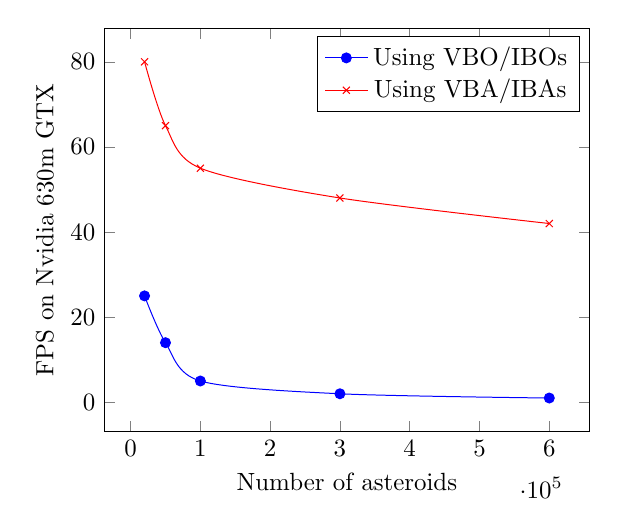
\begin{tikzpicture}[scale=0.9]
		\begin{axis}[
			xlabel=Number of asteroids,
			ylabel=FPS on Nvidia 630m GTX]
		\addplot[smooth,mark=*,blue] 
			plot coordinates {
			(20000,25.0)
			(50000,14.0)
			(100000,5.0)
			(300000,2.0)
			(600000,1.0)
		};
		\addlegendentry{Using VBO/IBOs}

		\addplot[smooth,color=red,mark=x]
			plot coordinates {
			(20000,80.0)
			(50000,65.0)
			(100000,55.0)
			(300000,48.0)
			(600000,42.0)
		};
		\addlegendentry{Using VBA/IBAs}
		\end{axis}
	\end{tikzpicture}
    \caption{Performance from 20,000 to 600,000 asteroids before and after implementing VBO/IBOs on an integrated Intel HD Graphics 3000 GPU}
    \label{FigVBOPerf}
  \end{center}
\end{figure}
\section{Graphics}
\label{secgraphics}

One of the main components of the simulation was of course the graphics. The main challenges
for this project were both making the graphics realistic and pleasing but also overcoming the
issues inherent with trying to render something with the scale of solar system. This section continues 
from the engine section but discusses specific graphics topics rather than the more general topics covered previously.

\subsection{Precision}
\label{precisionimpl}

Rendering objects at a realistic scale presented an issue due to the low precision
available on mobile GPUs when converting from double space to float space. This problem was solved by using a combination of two
methods. The coordinate system is first dynamically centred around the camera when
converting from double-space on the CPU side to float-space on the GPU side. This
eliminates the errors experienced when the camera is close to objects that are far from
the origin by always giving the highest level of precision to objects that are nearby.
Secondly, distant objects including those outside of the cameras clipping planes entirely
are scaled down and brought closer to the camera. This allows for objects to be any
distance away and still be visible but still be rendered at the correct size.

\subsubsection{Change of origin}

Due to the scene graph data structure shifting the origin of the entire scene is simple. All that is required is that the scene's root node's translation is set to the camera position before the scene update call. This change will automatically propagate the shift to all children. The change of origin must also be considered when passing parameters to the GPU and performing calculations on it since the shift will have already taken place. In many cases though, centring around the camera can actually eliminate instructions from being executing. For example the atmosphere shader (\cref{atmospheres}) requires the direction between a pixel and the camera. Normally this would mean normalising the difference between the pixel position and the camera position. Centred about the camera the camera position is always the zero vector so the result can be obtained just by normalising the position vector. This kind of technique is used many times throughout shaders and render call code and it is important to keep it in mind when evaluating the mathematics used in the shaders.

\subsubsection{Distant object scaling}

The second technique used was to develop an algorithm that transforms distant objects that would normally lie outside of the camera's clipping planes to be inside them and scaled down. This gives the same visual result as having an infinitely (up to the limit of double precision floating point numbers) large viewing distance.
\begin{align}
f = 0.5(c_f-c_n) \\
\overrightarrow{p}=f+f(1.0-e^{\frac{f-p_{real}}{p_{limit}}})\\
s=\frac{p}{p_{real}}
\end{align}
\vspace{-15pt} 
\begin{align*}
\text{where}~
\overrightarrow{p} &= \text{Position after transformation}  &
\overrightarrow{p_{real}} &= \text{Position before transformation}  \notag\\
\overrightarrow{p_{limit}} &= \text{Position before invisible}  &
f &= \text{Limit before scaling}  \notag\\
c_f &= \text{Far clipping plane} & c_n &= \text{Near clipping plane}  \notag\\
\end{align*}
\vspace{-25pt} 

\subsection{Stars}
\label{starfield}

Two solutions were considered for rendering stars. The first was to create a texture with the stars drawn on it using the right ascension and declination values in the star database and then map that texture over a sphere. The second was to use billboarding where each star is represented by a 3D quad angled at the camera where each quad can be pre-calculated. The second option was preferred as it allows for stars to be drawn with higher precision (Android has a texture size limit of 4096x4096 which results in visible artefacts). It would even allow the stars to be travelled to and still look acceptable with a suitable large texture being used. The process for creating these billboards is as follows:

\singlespacing
\begin{enumerate}
\item Take the star's Cartesian coordinates (provided light years) and normalise them to get a direction vector.
\item Take two cross products with the direction vector to get two perpendicular directions. The implementation uses a unit vector for the first product (it is safe to use the unit Y vector as no star lies precisely on that vector) and then finds the product of this new vector with direction vector.
\item Use these two vectors to calculate four vertices that create a square whose normal will be angled at the origin. The size of the square is based on the magnitude (\cref{starmagnitude}) of the star.
\item The vertices are also given a colour attribute which is calculated from the star's colour index and a texture coordinate. The colour will appropriately be blended with the star texture when rendered (explained later).
\item Project these four vertices along the direction vector so that their centre lies on the unit sphere.
\item Create two triangles from the square by referencing the four vertices using six indices which can then be rendered on the GPU.
\item Do this for all stars and add the resulting vertices/indices to a single VBO/IBO (\cref{vboibo}) respectively so only a single draw call to the GPU is required.
\item Translate all these points so that the sphere is centred on the camera on the GPU at render-time so that the quads face the camera rather than the origin.
\end{enumerate}
\onehalfspacing

Precisely, the position of each vertex for a single star can be calculated as follows (code for positions pre-transformation can be seen in \cref{codestargeom}):
\begin{align}
\mathbf{T}=\begin{pmatrix} 1 & 0 & 0 & c_x \\ 0 & 1 & 0 & c_y\\ 0 & 0 & 1 & c_z\\ 0 & 0 & 0 & 1 \end{pmatrix}\begin{pmatrix} v_{11} & v_{12} & v_{13} & 0 \\ v_{21} & v_{22} & v_{23} & 0\\ v_{31} & v_{32} & v_{33} & 0\\ 0 & 0 & 0 & 1 \end{pmatrix}\begin{pmatrix} p_{11} & p_{12} & p_{13} & p_{14} \\ p_{21} & p_{22} & p_{23} & p_{24}\\ p_{31} & p_{32} & p_{33} & p_{34}\\ p_{41} & p_{42} & p_{43} & p_{44} \end{pmatrix} \\
\overrightarrow{v_0}=\mathbf{T}[\widehat{p}+(-s(\widehat{p}\times\widehat{y})+s(\widehat{p}\times(\widehat{p}\times\widehat{y})))] \\
\overrightarrow{v_1}=\mathbf{T}[\widehat{p}+(-s(\widehat{p}\times\widehat{y})-s(\widehat{p}\times(\widehat{p}\times\widehat{y})))] \\
\overrightarrow{v_2}=\mathbf{T}[\widehat{p}+(s(\widehat{p}\times\widehat{y})+s(\widehat{p}\times(\widehat{p}\times\widehat{y})))] \\
\overrightarrow{v_3}=\mathbf{T}[\widehat{p}+(s(\widehat{p}\times\widehat{y})-s(\widehat{p}\times(\widehat{p}\times\widehat{y})))]
\end{align}
\vspace{-55pt} 
\singlespacing
\begin{align*}
\text{where}~\mathbf{T} &= \text{Final transformation matrix,} \notag\\
\mathbf{V} &= \text{View matrix} \notag\\
\mathbf{P} &= \text{Projection matrix} \notag\\
\overrightarrow{p} &= \text{Star position} \notag\\
\widehat{p} &= \text{Normalised star position} \notag\\
\widehat{y} &= \text{Unit y vector} \notag\\
s &= \text{Star scale}\notag
\end{align*}
\onehalfspacing
\vspace{-25pt} 

\begin{figure}[!htbp]
\centering
\begin{subfigure}{.5\textwidth}
  \centering
  \includegraphics[width=.98\linewidth]{starsphere0}
  \caption{Internal view}
  \label{fig:starsphereint0}
\end{subfigure}%
\begin{subfigure}{.5\textwidth}
  \centering
  \includegraphics[width=.98\linewidth]{starsphere1}
  \caption{External view}
  \label{fig:starsphereext0}
\end{subfigure}
\caption{Star sphere shown from different views (star sizes greatly increased for clarity).}
\label{fig:stars1}
\end{figure}

\begin{figure}[!htbp]
\centering
\begin{subfigure}{.5\textwidth}
  \centering
  \includegraphics[width=.98\linewidth]{starsphere2}
  \caption{Internal view}
  \label{fig:starsphereint1}
\end{subfigure}%
\begin{subfigure}{.5\textwidth}
  \centering
  \includegraphics[width=.98\linewidth]{starsphere3}
  \caption{External view}
  \label{fig:starsphereext1}
\end{subfigure}
\caption{Star sphere textured shown from different views (star sizes greatly increased for clarity).}
\label{fig:stars2}
\end{figure}

\begin{figure}[!htbp]
\centering
\begin{subfigure}{.5\textwidth}
  \centering
  \includegraphics[width=.98\linewidth]{starsphere4}
  \caption{Internal view}
  \label{fig:starsphereint2}
\end{subfigure}%
\begin{subfigure}{.5\textwidth}
  \centering
  \includegraphics[width=.98\linewidth]{starsphere5}
  \caption{External view}
  \label{fig:starsphereext2}
\end{subfigure}
\caption{Star sphere final render quality with texturing, colouring and correct scaling.}
\label{fig:stars3}
\end{figure}

\subsection{Dynamic LOD (Level of Detail)}

To ensure that planets and other bodies appear to be perfectly spherical a relatively high vertex count is required. These high vertex counts result in a heavy load on the rather unpowerful mobile GPUs and would mean that there would be considerably slowdowns when drawing multiple bodies. However, due to the scale of galactic bodies and the astronomical distances between them, only one or at most a few spherical entities need to be drawn with a particularly high level of detail. So therefore a metric was derived that queries the engine to provide a suitably detailed sphere for an object of given distance from the camera and scale. This in combination with frustum culling were key in achieving a high frame-rate on mobile GPUs.

\begin{figure}[!htbp]
\centering
\begin{subfigure}{.33\textwidth}
  \centering
  \includegraphics[width=.98\linewidth]{lod0}
  \caption{LOD 0 (unused)}
  \label{fig:lod0}
\end{subfigure}%
\begin{subfigure}{.33\textwidth}
  \centering
  \includegraphics[width=.98\linewidth]{lod1}
  \caption{LOD 1}
  \label{fig:lod1}
\end{subfigure}%
\begin{subfigure}{.33\textwidth}
  \centering
  \includegraphics[width=.98\linewidth]{lod2}
  \caption{LOD 2}
  \label{fig:lod2}
\end{subfigure}
\begin{subfigure}{.33\textwidth}
  \centering
  \includegraphics[width=.98\linewidth]{lod3}
  \caption{LOD 3}
  \label{fig:lod3}
\end{subfigure}
\begin{subfigure}{.33\textwidth}
  \centering
  \includegraphics[width=.98\linewidth]{lod4}
  \caption{LOD 4}
  \label{fig:lod4}
\end{subfigure}
\caption{Star sphere final render quality with texturing, colouring and correct scaling.}
\label{fig:lods}
\end{figure}

\subsection{Bitmap font based text}
\label{bitmapfont}

The ability to display text on screen is required to show the names of solar bodies and stars. One of the fastest ways to to do this is to use a bitmap font based rendering system. 
A bitmap font is an image with all the character glyphs rastered at particular size. 
The position of each character is known either by having a map or simply by storing the characters in the standard ASCII order (we use this approach). 
To render text using the GPU, this bitmap font is uploaded and then quads are sent to be rendered in the correct position with the texture coordinates pre-calculated to point to the appropriate character in the texture. 
These quads can be transformed in the same way that any other geometry can. This allows for example, showing text in 2D to display debug information, or positioning text above galactic entities to show their names.
The bitmap font class provides the ability to update the underlying VBOs and IBOs (\cref{vboibo}) so that text can be efficiently be changed on every draw call if desired. Our debug information text for example was set to update every 10ms with a new value for framerate, position and so on.
\\
\begin{figure}[!htbp]
  \begin{center}
    \leavevmode
    \ifpdf
      \includegraphics[width=1\textwidth]{text0}
    \fi
    \caption{Geometry underlying the rendering of text}
    \label{FigText0}
  \end{center}
\end{figure}

\begin{figure}[!htbp]
  \begin{center}
    \leavevmode
    \ifpdf
      \includegraphics[width=1\textwidth]{text1}
    \fi
    \caption{Texture overlayed over the geometry with texture coordinates pointing to particular characters to produce the desired text output.}
    \label{FigText1}
  \end{center}
\end{figure}

Note how this technique is essentially the same as was used to render stars, only with varying texture coordinates and different transformations.

\subsection{Shaders}

Modern graphics APIs (OpenGL 2.0 onwards and DirectX 8 onwards) in conjunction with modern GPUs use a programmable graphics pipeline where shader programs rather than fixed functions are used to produce screen output from geometry, textures and so on. On OpenGL ES 2.0, the type of shaders available are vertex shaders and pixel shaders. Vertex shaders transform vertex data into screen space and perform any other per-vertex calculations the developer desires. Pixel shaders take the output from vertex shaders and 'fill in the gaps' by calculating the colour and depth value of every pixel on the screen using interpolation between vertices and user specified per-pixel calculations. As a general rule, there are many times less vertex operations than pixel operations and there is sometimes a choice whether or not to perform a task per-vertex or per-pixel. An example of this would be for the fractal texturing of the Sun's surface (\cref{fractalstar}). If the colour is calculated per vertex, then the pixels in-between will be interpolated. If the value is instead calculated per pixel then the fractal calculation is performed many more times. This results in a much higher quality output but is far more costly.

\subsection{Fractal-based star surface shader}
\label{fractalstar}

To simulate the volatile surface of the sun, we used a GLSL library that generates 3D simplex noise. By providing the simulation time as one of the arguments, this results in an animated and convincing looking colouring. A problem was encountered with getting this running at an acceptable speed on the mobile GPUs available to the group. Doing the calculation on the pixel shader slowed down the simulation to running at around 5-10 frames per second (down from around 45). This is clearly unacceptable, so next we attempted to do the calculations per vertex which having tested on PC version, should have made the performance impact far lower. The visuals were also still pleasing enough for the smaller mobile screens. Unfortunately we discovered that current generation mobile GPUs have a low instruction limit for vertex shaders (the Mali-400 GPU on the Samsung N7000 had a limit of 512 instructions whereas the shader was nearly 3000 instructions). As such this effect is currently disabled on the mobile version, but should be compatible with the current top-end devices and certainly future ones.

\begin{figure}[!htbp]
\centering
\begin{minipage}{.5\textwidth}
  \centering
  \includegraphics[width=.98\linewidth]{star_per_pixel}
  \caption{Shader applied per-pixel}
  \label{fig:spp}
\end{minipage}%
\begin{minipage}{.5\textwidth}
  \centering
  \includegraphics[width=.98\linewidth]{star_per_vertex}
  \caption{Shader applied per-vertex}
  \label{fig:spv}
\end{minipage}
\end{figure}

\subsection{Atmospheric shaders}
\label{atmospheres}

The atmospheric and corona shaders are by far the most complex in our application. The process of calculating the colour for a given pixel is mathematically intensive and to show all the details is out of the scope of this report (although the full source will be available in our submission for those interested). 

\begin{figure}[!htbp]
  \begin{center}
    \leavevmode
    \ifpdf
      \includegraphics[width=0.5\textwidth]{atmos_diag1}
    \fi
    \caption{Atmosphere sphere drawn over the planet sphere}
    \label{FigAtmosDiag1}
  \end{center}
\end{figure}

At a very high level, the shader works by drawing a second sphere with a radius greater than that of the planet surface. Knowing the radius of both the atmosphere and the surface, the shader then calculates the height ($h$) of a given vertex ($V_0$) above the planets surface as the vertex appears to the \textbf{camera} by finding the point of intersection of a ray cast from the camera with the atmosphere geometry followed by a number of other calculations. A transparency value is also calculated and the rendering is done with blending enabled to give a realistic final effect.

\subsubsection{Corona shader}

The corona shader shares the majority of its code with the atmosphere shader. It additionally deforms sphere vertices using the same fractal noise function described in \cref{fractalstar} and applies a gradient colour rather than a single colour. This gives a more realistic impression of the Sun's Corona than having a still effect. However, as with the Sun surface shader, the number of vertex shader instructions required was greater than available on the phones we had available to test on so it is currently only available on the PC version.

\begin{figure}[!htbp]
\centering
\begin{minipage}{.5\textwidth}
  \centering
  \includegraphics[width=.98\linewidth]{atmos}
  \caption{Atmosphere shader}
  \label{fig:atmos}
\end{minipage}%
\begin{minipage}{.5\textwidth}
  \centering
  \includegraphics[width=.98\linewidth]{corona}
  \caption{Corona shader}
  \label{fig:corona}
\end{minipage}
\end{figure}

\begin{figure}[!htbp]
\centering
\begin{subfigure}{.5\textwidth}
  \centering
  \includegraphics[width=.98\linewidth]{corona2}
  \label{fig:corona2}
\end{subfigure}%
\begin{subfigure}{.5\textwidth}
  \centering
  \includegraphics[width=.98\linewidth]{corona3}
  \label{fig:corona3}
\end{subfigure}
\caption{The noise amount can be customised which allows for interesting effects.}
\label{fig:coronafull}
\end{figure}

\pagebreak
\subsection{Asteroid shader}
In order to draw a massive number of asteroids - up to the six hundred thousand that are available in the NASA small body database - the orbital physics code was ported to GLSL. Instead of passing geometry to the vertex shader as with all other shaders, the orbital data of all the asteroids are sent instead (using a single VBO - \cref{vboibo}) and the shader calculates a single point representing the position of the asteroid. Textured point sprites (very similar to how stars are rendered - section{starfield}) are then used to render the asteroids. We experimented with using a realistic asteroid texture and an entirely false one. Neither produced a particularly realistic view of the asteroids and we felt the false view was more pleasing and allowed the user to better appreciate the sheer number of objects that exist in the asteroid belt. The next generation of phones will have hardware instancing and geometry shader support which will allow for the efficient rendering of the calculated points with real geometry. The full code for the vertex shader has been included in \cref{asteroidshadercode}.

\begin{figure}[!htbp]
\centering
\begin{minipage}{.5\textwidth}
  \centering
  \includegraphics[width=.98\linewidth]{asteroids_20k}
  \caption{20,000 asteroids}
  \label{fig:ast1}
\end{minipage}%
\begin{minipage}{.5\textwidth}
  \centering
  \includegraphics[width=.98\linewidth]{asteroids_600k}
  \caption{Full 600,000 asteroids}
  \label{fig:ast2}
\end{minipage}
\end{figure}
\vspace{-12pt}
\begin{figure}[!htbp]
  \begin{center}
    \leavevmode
    \ifpdf
      \includegraphics[width=0.45\textwidth]{asteroids_20k_real}
    \fi
    \caption{20,000 asteroids rendered with a realistic texture}
    \label{fig:ast3}
  \end{center}
\end{figure}

\subsection{Planetary shaders}

The complexity of all shaders are slightly limited by the comparatively outdated mobile GPUs. Despite this, we have achieved a quality of rendering unmatched by any of the existing solutions that we tested by combining the atmospheric effects with relatively advanced planetary shaders and shadowing techniques. They use techniques such as diffuse lighting, bump mapping and specular highlights to give depth and realistic lighting to the planets surface. The only technique we implemented that would not run on current mobile GPUs was heightmapping where each vertex on the sphere is transformed in line with the terrain height by querying a height texture. This was not possible as texture lookups in the vertex shader are not possible with the current Android GLSL implementation. This is another feature along with the star surface shader we can enable as the next generation of phones become available.

\subsubsection{Building the Earth - Diffuse lighting}

\begin{figure}[!htbp]
\centering
  \centering
  \includegraphics[width=.5\linewidth]{diffuse1}
  \caption{Diffuse lighting on a flat surface}
  \label{fig:diffuse1}
\end{figure}

Diffuse lighting is a simple direct lighting method that takes no consideration of the eye position and works by calculating the intensity of light reflected by part of an object as a function of a objects's orientation toward a light source.
The diffuse lighting in our application works by calculating the dot product of the surface normal at a particular pixel with the direction of the light source. This value is clamped in the interval [0,1] and then multiplied by the diffuse texture to produce the final diffuse colour contribution.
Additionally, distance attenuation is performed to show that the intensity of light diminishes the further an object is from a light source. Our implementation of this does not use realistic values as the results are no longer visual pleasing to the user when doing so. Instead the light intensity halves by the time Pluto is reached, which gives the desired impression without making the scene too dark for the user.
The mathematics for this method is as follows:
\vspace{-10pt} 
\begin{align}
\widehat{l} = \overrightarrow{p_{sol}}-\overrightarrow{p_{pixel}} \\
a = 0.5+0.5\times \dfrac{min(\|\overrightarrow{p_{pixel}}\|_2, 0)}{50}  \\
d = \begin{cases} (\widehat{l} \cdot \widehat{n})  &\mbox{if } (\widehat{l} \cdot \widehat{n}) \ge 0 \\ 
\overrightarrow{0} & \mbox{if } (\widehat{l} \cdot \widehat{n}) < 0 \end{cases} \\
\overrightarrow{c_{diff}} = ad \times \overrightarrow{t_{diff-day}}
\end{align}
\vspace{-40pt} 
\begin{align*}
\text{where}~
\widehat{l} &= \text{Light direction to pixel} \notag\\
\overrightarrow{p_{pixel}} &= \text{Pixel position (world space)} \notag\\
\overrightarrow{p_{sol}} &= \text{Sol position (world space)} \notag\\
\widehat{n} &= \text{Surface normal at pixel (world space)} \notag\\
\overrightarrow{t_{diff-day}} &= \text{Day texture sample colour} \notag\\
\overrightarrow{c_{diff}} &= \text{Diffuse colour} \notag\\
d &= \text{Diffuse amount} \notag\\
a  &= \text{Distance attenuation} \notag\\
\end{align*}
\vspace{-45pt}

\begin{figure}[!htbp]
\centering
\begin{minipage}{.5\textwidth}
  \centering
  \includegraphics[width=.98\linewidth]{earth1}
  \caption{Textured sphere}
  \label{fig:earth1}
\end{minipage}%
\begin{minipage}{.5\textwidth}
  \centering
  \includegraphics[width=.98\linewidth]{earth2}
  \caption{Diffuse lighting added}
  \label{fig:earth2}
\end{minipage}
\end{figure}

\pagebreak
\subsubsection{Building the Earth - Day/night earth shading}

Unique to the Earth is the requirement to have separate day and night textures due to human lights being visible at night. 
To determine the final colour of a pixel, add to the diffuse colour value previously calculated 
a proportion of the night texture colour depending on the inverse value of the diffuse lighting amount. We give a bias towards the day texture since a location with say 90\% of full day sunlight will not have lights turned on. 
So rather than doing a full inverse (i.e. $1.0-d$) we used the value of $2.0(max(0.5-d,0.0)$ to make the night texture start being blended in at 50\% of full daylight.

\vspace{-10pt} 
\begin{align}
\overrightarrow{c_{diff}} = (ad \times \overrightarrow{t_{diff-day}})+2.0(max((0.5-d), 0.0))\times \overrightarrow{t_{diff-night}})
\end{align}
\vspace{-40pt} 
\begin{align*}
\text{where}~
\overrightarrow{t_{diff-day}} &= \text{Day texture sample colour} \notag\\
\overrightarrow{t_{diff-night}} &= \text{Night texture sample colour} \notag\\
\overrightarrow{c_{diff}} &= \text{Diffuse colour} \notag\\
d &= \text{Diffuse amount} \notag\\
a  &= \text{Distance attenuation} \notag\\
\end{align*}
\vspace{-45pt} 

\begin{figure}[!htbp]
\centering
\begin{minipage}{.5\textwidth}
  \centering
  \includegraphics[width=.98\linewidth]{earth3a}
  \caption{Day/night texture added}
  \label{fig:earth3a}
\end{minipage}%
\begin{minipage}{.5\textwidth}
  \centering
  \includegraphics[width=.98\linewidth]{earth3b}
  \caption{Dark side of the Earth}
  \label{fig:earth3b}
\end{minipage}
\end{figure}

\pagebreak
\subsubsection{Building the Earth - Dot3 bump mapping}

Dot3 bump mapping also known as normal mapping is a technique commonly used in games (although it is now being surpassed by other techniques at the cutting edge with desktop GPUs) to give the impression of a higher detailed geometry than what is actually being used. The result is convincing because it also simulates how the lighting would effect this higher-detailed geometry. The process we use is very similar to the standard techniques so a detailed explanation will not be given in this report. The full shader and CPU-side code will be available in our source submission however.

\begin{figure}[!htbp]
\centering
\begin{minipage}{.5\textwidth}
  \centering
  \includegraphics[width=.98\linewidth]{earth_normal}
  \caption{Earth normal map}
  \label{fig:earth4a}
\end{minipage}%
\begin{minipage}{.5\textwidth}
  \centering
  \includegraphics[width=.98\linewidth]{earth4}
  \caption{Dot3 bump mapping applied}
  \label{fig:earth4b}
\end{minipage}
\end{figure}

\subsubsection{Building the Earth - Specular highlights}

Specular highlights are used to show the reflection of light from the Earth's Oceans. This is a fairly simple process and involves using a specular texture map to specify which areas of the surface are reflective (i.e. the oceans) and calculating the points where the light is most intense by taking powers of the values calculated in the diffuse lighting process.

\begin{figure}[!htbp]
\centering
\begin{minipage}{.5\textwidth}
  \centering
  \includegraphics[width=.98\linewidth]{earth_specmap}
  \caption{Earth specular map}
  \label{fig:earth5a}
\end{minipage}%
\begin{minipage}{.5\textwidth}
  \centering
  \includegraphics[width=.98\linewidth]{earth5}
  \caption{Specular highlights applied}
  \label{fig:earth5b}
\end{minipage}
\end{figure}

\pagebreak
\subsubsection{Building the Earth - Height maps}
\label{heightmaps}

The vertex shader for planets has support for offsetting the vertices of the planet surface by an amount depending on the value from a sampled monochrome image. Since the sphere is centred around the origin in object space, this offsetting process is mathematically very straightforward:

\singlespacing
\vspace{-25pt}
\begin{align}
h = sample(heightTexture, \overrightarrow{uv}) \\
\overrightarrow{off} = \widehat{n} \times s \times h \\
\overrightarrow{P_v} = \overrightarrow{P_v} + \overrightarrow{off} 
\end{align}
\vspace{-10pt}
\begin{align*}
\text{where}~
h &= \text{Height sample value} \notag\\
s &= \text{Height scale factor} \notag\\
\widehat{n} &= \text{Vertex normal vector in object space} \notag\\
\overrightarrow{P_v} &= \text{Vertex position in object space (initial value sent by application to GPU)} \notag\\
\overrightarrow{uv} &= \text{Texture coordinate input (same as for surface texture)} \notag\\
\end{align*}
\vspace{-35pt}
\onehalfspacing

However, the sampling textures in the vertex shader is not supported on the current generation of Android phones (it will be on the next) so the effect is disabled but it does function on the PC version.
\\
\begin{figure}[!htbp]
\centering
\begin{subfigure}{.5\textwidth}
  \centering
  \includegraphics[width=.98\linewidth]{earth_heightmap}
  \caption{From high orbit}
  \label{fig:earthhm1}
\end{subfigure}%
\begin{subfigure}{.5\textwidth}
  \centering
  \includegraphics[width=.98\linewidth]{earth_heightmap2}
  \caption{From lower orbit}
  \label{fig:earthhm2}
\end{subfigure}
\caption{Heightmapping on Earth (scale has been greatly increased for clarity).}
\label{fig:earthhms2}
\end{figure}

\subsubsection{Building the Earth - Cloud layer}

The clouds are rendered simply by drawing a slightly larger sphere over the Earth's surface with a transparent cloud texture applied over it.

\begin{figure}[!htbp]
\centering
\begin{minipage}{.5\textwidth}
  \centering
  \includegraphics[width=.98\linewidth]{earth6}
  \caption{Cloud layer added}
  \label{fig:earth6}
\end{minipage}%
\begin{minipage}{.5\textwidth}
  \centering
  \includegraphics[width=.98\linewidth]{earth7}
  \caption{Atmosphere enabled}
  \label{fig:earth7}
\end{minipage}
\end{figure}

\pagebreak
\subsection{Plantary rings}
\label{planetaryrings}

At this point mobile GPUs do not have geometry shaders and have limited support for hardware geometry instancing so it was unrealistic
to attempt drawing planetary rings in a completely realistic way. Instead our implementation uses a texture with alpha transparency applied to a quad
to give a good impression of the planetary rings. The only time where this method does not look convincing is if the user is in the same plane as the quad in which case the rings are not visible, but this is a trade-off with using this method. Rather than using one large texture that contains an image of the entire rings, we use a texture that only represents a small segment of the rings.

\begin{figure}[!htbp]
\centering
  \centering
  \includegraphics[width=1.0\linewidth]{saturn_rings}
  \caption{Source texture for Saturn's Rings with transparency shown as black.}
  \label{fig:satrings}
\end{figure}

This texture is applied to the plane by calculating texture coordinates per pixel in a pixel shader based on distance from the centre of the planet. Doing this allows for a much higher detail texture to be used than if using a single texture for the entire ring entity (texture size limit on Android is currently 4096x4096 and this method simulates a texture size many times larger than this). To determine what part of the image to sample from for a given pixel:

\singlespacing
\vspace{-10pt}
\begin{align}
m = \dfrac{1.0}{1.0-f} \\
u = max(\|\overrightarrow{P_v}\|_2-f,0.0)\times m \\
\overrightarrow{uv} =\begin{pmatrix}
 u \\ 
 0.5
 \end{pmatrix}
\end{align}
\vspace{-10pt}
\begin{align*}
\text{where}~
u &= \text{U texture coordinate} \notag\\
f &= \text{Percentage distance to start ring texture in [0,1]} \notag\\
m &= \text{Scaling factor for U coordinate} \notag\\
\overrightarrow{P_v} &= \text{Pixel position in object space} \notag\\
\overrightarrow{uv} &= \text{Day texture sample colour} \notag\\
\end{align*}
\vspace{-25pt}

\begin{figure}[!htbp]
\centering
\begin{minipage}{.5\textwidth}
  \centering
  \includegraphics[width=.98\linewidth]{rings1}
  \caption{Rings of Saturn}
  \label{fig:rings1}
\end{minipage}%
\begin{minipage}{.5\textwidth}
  \centering
  \includegraphics[width=.98\linewidth]{rings2}
  \caption{Rings of Neptune}
  \label{fig:rings2}
\end{minipage}
\end{figure}
\onehalfspacing

\pagebreak
\subsection{Shadowing}

A requirement was that the solar system should be rendered at an accurate scale
and that objects cast shadows so that eclipses will be realistically represented. Our implementation
additionally renders the shadows cast by planets on their planetary rings (\cref{planetaryrings}). The
common methods for rendering shadows tend to be either approximations that would
not have worked well at such scales or be too computationally intensive to run on a
mobile device. The solution to this was to use a take on ray casting which is optimised
for the spherical planet objects and does not account for reflected light, only that
which comes directly from the Sun.

\subsubsection{Ray casting}

The implementation for eclipse shadowing works by casting three rays which enable finding the umbra and penumbra radii. These rays go from the centre of the Sun through Luna to find the umbra centre, from an edge of the Sun over the same edge on the Moon to find a point on the umbra/penumbra boundary and from an edge of the Sun over the opposite edge on the Moon to find the point where the penumbra ends. These two radii are
set on each render call to the GPU. From there a ray is calculated from the centre of the Sun through the centre of Luna on the GPU and in the pixel shader the distance of each pixel from this ray is found. If it lies within the umbra radius, the pixel colour becomes fully black. If it lies within the penumbra then the black intensity is calculated based on how far from the umbra the point is.

\begin{figure}[!htbp]
\centering
  \centering
  \includegraphics[width=1.0\linewidth]{shadow_diag}
  \caption{Diagram shows the three rays cast (six here as it is done on both sides)}
  \label{fig:shadowd1}
\end{figure}

\begin{figure}[!htbp]
\centering
\begin{minipage}{.5\textwidth}
  \centering
  \includegraphics[width=.98\linewidth]{shadow_diag2}
  \caption{Radii used in calculations}
  \label{fig:shadowd2}
\end{minipage}%
\begin{minipage}{.5\textwidth}
  \centering
  \includegraphics[width=.98\linewidth]{shadow_diag3}
  \caption{Resulting effect}
  \label{fig:shadowd3}
\end{minipage}
\end{figure}

Mathematically, the process of calculating the shadow attenuation for each pixel for eclipses is:

\singlespacing
\begin{align}
\widehat{l} =\dfrac{ \overrightarrow{P_{Luna}}-\overrightarrow{P_{Sol}}}{ \| \overrightarrow{P_{Luna}}-\overrightarrow{P_{Sol}}\|_2} \\
d = \| (\overrightarrow{P_{Luna}}-\overrightarrow{P_{p}}) \times \widehat{l} \|_2 \\
a = clamp(\dfrac{d - r_u}{r_p - r_u}, 0.0, 1.0)
\end{align}
\begin{align*}
\text{where}~
r_u &= \text{Umbra radius projected from Luna} \notag\\
r_p &= \text{Penumbra radius projected from Luna} \notag\\
\widehat{l} &= \text{Light ray direction} \notag\\
\overrightarrow{P_{Luna}} &= \text{Position of Luna in world space} \notag\\
\overrightarrow{P_{Sol}} &= \text{Position of Sol in world space} \notag\\
\overrightarrow{P_{p}} &= \text{Position of pixel in world space} \notag\\
d &= \text{Distance of pixel from ray cast from Sol to Luna} \notag\\
a &= \text{Shadow attenuation} \notag\\
\end{align*}
\onehalfspacing

\pagebreak

The process for shadowing planetary rings is similar. The difference is that instead of calculating the umbra and penumbra radius based off rays cast from the Sun through the Moon, the umbra radius is set simply to the radius of the planet and the penumbra radius is set to a scaled up planet radius. Images of the resulting effect can be seen in \cref{planetaryrings}. The mathematics for shadow attenuation now becomes:

\singlespacing
\begin{align}
f = \dfrac{1.0}{s_p-1.0} \\
\widehat{l} =\dfrac{ \overrightarrow{P_{Planet}}-\overrightarrow{P_{Sol}}}{ \| \overrightarrow{P_{Planet}}-\overrightarrow{P_{Sol}}\|_2} \\
d = \| (\overrightarrow{P_{Planet}}-\overrightarrow{P_{p}}) \times \widehat{l} \|_2 \\
a = \begin{cases} clamp(\dfrac{fd}{r}-f, 0.1, 1.0)  &\mbox{if } \|\overrightarrow{P_{p}}-\overrightarrow{P_{Sol}}\|_2 > \|\overrightarrow{P_{Planet}}-\overrightarrow{P_{Sol}}\|_2 \\ 
\overrightarrow{1.0} & \mbox{otherwise} \end{cases} \\
\end{align}

\begin{align*}
\text{where}~
s_p &= \text{Penumbra scale, value of 1.2 is used currently} \notag\\
f &= \text{Inverse scaling difference} \notag\\
r &= \text{Planet radius} \notag\\
\widehat{l} &= \text{Light ray direction} \notag\\
\overrightarrow{P_{Planet}} &= \text{Position of casting planet in world space} \notag\\
\overrightarrow{P_{Sol}} &= \text{Position of Sol in world space} \notag\\
\overrightarrow{P_{p}} &= \text{Position of pixel in world space} \notag\\
d &= \text{Distance of pixel from ray cast from Sol to Luna} \notag\\
a &= \text{Shadow attenuation} \notag\\
\end{align*}
\onehalfspacing